\documentclass[twoside]{book}

% Packages required by doxygen
\usepackage{fixltx2e}
\usepackage{calc}
\usepackage{doxygen}
\usepackage[export]{adjustbox} % also loads graphicx
\usepackage{graphicx}
\usepackage[utf8]{inputenc}
\usepackage{makeidx}
\usepackage{multicol}
\usepackage{multirow}
\PassOptionsToPackage{warn}{textcomp}
\usepackage{textcomp}
\usepackage[nointegrals]{wasysym}
\usepackage[table]{xcolor}

% Font selection
\usepackage[T1]{fontenc}
\usepackage[scaled=.90]{helvet}
\usepackage{courier}
\usepackage{amssymb}
\usepackage{sectsty}
\renewcommand{\familydefault}{\sfdefault}
\allsectionsfont{%
  \fontseries{bc}\selectfont%
  \color{darkgray}%
}
\renewcommand{\DoxyLabelFont}{%
  \fontseries{bc}\selectfont%
  \color{darkgray}%
}
\newcommand{\+}{\discretionary{\mbox{\scriptsize$\hookleftarrow$}}{}{}}

% Page & text layout
\usepackage{geometry}
\geometry{%
  a4paper,%
  top=2.5cm,%
  bottom=2.5cm,%
  left=2.5cm,%
  right=2.5cm%
}
\tolerance=750
\hfuzz=15pt
\hbadness=750
\setlength{\emergencystretch}{15pt}
\setlength{\parindent}{0cm}
\setlength{\parskip}{3ex plus 2ex minus 2ex}
\makeatletter
\renewcommand{\paragraph}{%
  \@startsection{paragraph}{4}{0ex}{-1.0ex}{1.0ex}{%
    \normalfont\normalsize\bfseries\SS@parafont%
  }%
}
\renewcommand{\subparagraph}{%
  \@startsection{subparagraph}{5}{0ex}{-1.0ex}{1.0ex}{%
    \normalfont\normalsize\bfseries\SS@subparafont%
  }%
}
\makeatother

% Headers & footers
\usepackage{fancyhdr}
\pagestyle{fancyplain}
\fancyhead[LE]{\fancyplain{}{\bfseries\thepage}}
\fancyhead[CE]{\fancyplain{}{}}
\fancyhead[RE]{\fancyplain{}{\bfseries\leftmark}}
\fancyhead[LO]{\fancyplain{}{\bfseries\rightmark}}
\fancyhead[CO]{\fancyplain{}{}}
\fancyhead[RO]{\fancyplain{}{\bfseries\thepage}}
\fancyfoot[LE]{\fancyplain{}{}}
\fancyfoot[CE]{\fancyplain{}{}}
\fancyfoot[RE]{\fancyplain{}{\bfseries\scriptsize Generated by Doxygen }}
\fancyfoot[LO]{\fancyplain{}{\bfseries\scriptsize Generated by Doxygen }}
\fancyfoot[CO]{\fancyplain{}{}}
\fancyfoot[RO]{\fancyplain{}{}}
\renewcommand{\footrulewidth}{0.4pt}
\renewcommand{\chaptermark}[1]{%
  \markboth{#1}{}%
}
\renewcommand{\sectionmark}[1]{%
  \markright{\thesection\ #1}%
}

% Indices & bibliography
\usepackage{natbib}
\usepackage[titles]{tocloft}
\setcounter{tocdepth}{3}
\setcounter{secnumdepth}{5}
\makeindex

% Hyperlinks (required, but should be loaded last)
\usepackage{ifpdf}
\ifpdf
  \usepackage[pdftex,pagebackref=true]{hyperref}
\else
  \usepackage[ps2pdf,pagebackref=true]{hyperref}
\fi
\hypersetup{%
  colorlinks=true,%
  linkcolor=blue,%
  citecolor=blue,%
  unicode%
}

% Custom commands
\newcommand{\clearemptydoublepage}{%
  \newpage{\pagestyle{empty}\cleardoublepage}%
}

\usepackage{caption}
\captionsetup{labelsep=space,justification=centering,font={bf},singlelinecheck=off,skip=4pt,position=top}

%===== C O N T E N T S =====

\begin{document}

% Titlepage & ToC
\hypersetup{pageanchor=false,
             bookmarksnumbered=true,
             pdfencoding=unicode
            }
\pagenumbering{roman}
\begin{titlepage}
\vspace*{7cm}
\begin{center}%
{\Large My Project }\\
\vspace*{1cm}
{\large Generated by Doxygen 1.8.11}\\
\end{center}
\end{titlepage}
\clearemptydoublepage
\tableofcontents
\clearemptydoublepage
\pagenumbering{arabic}
\hypersetup{pageanchor=true}

%--- Begin generated contents ---
\chapter{File Index}
\section{File List}
Here is a list of all files with brief descriptions\+:\begin{DoxyCompactList}
\item\contentsline{section}{src/\hyperlink{_detection_8cpp}{Detection.\+cpp} \\*Implements class Implementation }{\pageref{_detection_8cpp}}{}
\item\contentsline{section}{src/\hyperlink{_detection_main_8cpp}{Detection\+Main.\+cpp} \\*Main file for Detection node }{\pageref{_detection_main_8cpp}}{}
\item\contentsline{section}{src/\hyperlink{main_8cpp}{main.\+cpp} }{\pageref{main_8cpp}}{}
\item\contentsline{section}{src/\hyperlink{_navigation_8cpp}{Navigation.\+cpp} \\*Navigation class Implementation }{\pageref{_navigation_8cpp}}{}
\item\contentsline{section}{src/\hyperlink{_navigation_main_8cpp}{Navigation\+Main.\+cpp} \\*Main file for Navigation node }{\pageref{_navigation_main_8cpp}}{}
\item\contentsline{section}{src/\hyperlink{_user_interface_8cpp}{User\+Interface.\+cpp} \\*Implements User\+Interface class }{\pageref{_user_interface_8cpp}}{}
\item\contentsline{section}{src/\hyperlink{_warehouse_manager_8cpp}{Warehouse\+Manager.\+cpp} \\*Implements Warehouse\+Manager class }{\pageref{_warehouse_manager_8cpp}}{}
\end{DoxyCompactList}

\chapter{File Documentation}
\hypertarget{_detection_8cpp}{}\section{src/\+Detection.cpp File Reference}
\label{_detection_8cpp}\index{src/\+Detection.\+cpp@{src/\+Detection.\+cpp}}


Implements class Implementation.  


{\ttfamily \#include \char`\"{}../include/\+Detection.\+hpp\char`\"{}}\\*
{\ttfamily \#include \char`\"{}../include/\+I\+Detection.\+hpp\char`\"{}}\\*
Include dependency graph for Detection.\+cpp\+:
\nopagebreak
\begin{figure}[H]
\begin{center}
\leavevmode
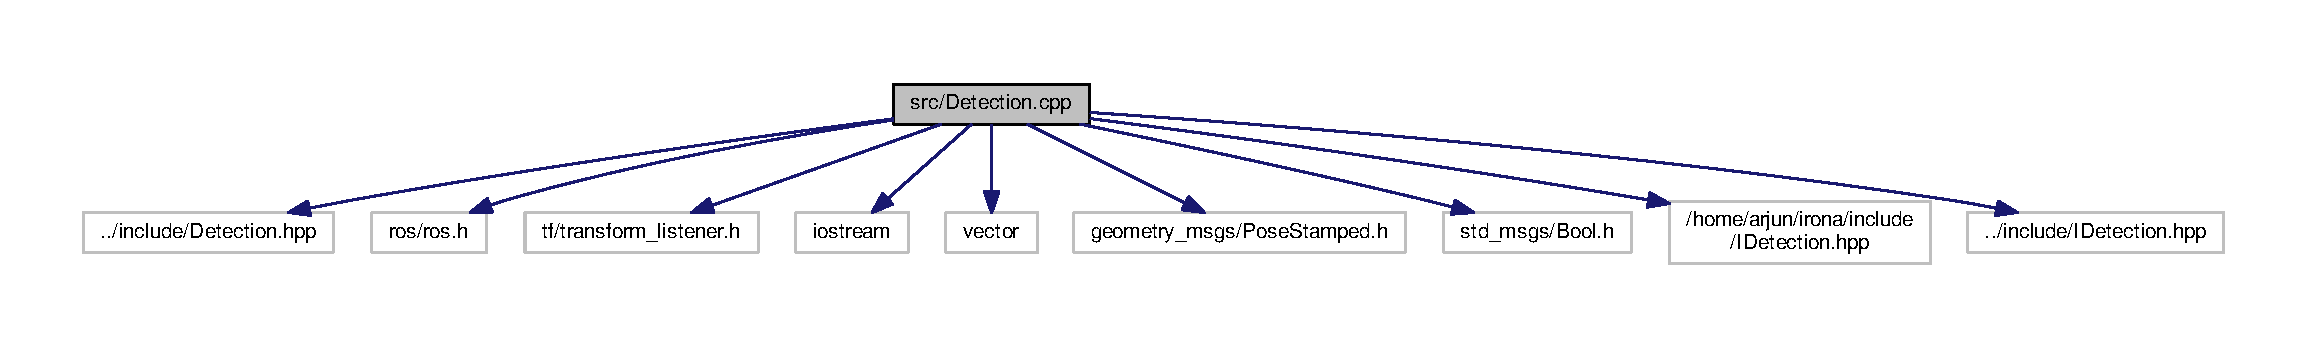
\includegraphics[width=350pt]{_detection_8cpp__incl}
\end{center}
\end{figure}


\subsection{Detailed Description}
Implements class Implementation. 

\begin{DoxyAuthor}{Author}
Kartik Madhira 

Arjun Gupta 

Aruna Baijal 
\end{DoxyAuthor}
\begin{DoxyCopyright}{Copyright}
M\+IT License (c) 2019 Kartik Madhira, Aruna Baijal, Arjun Gupta 
\end{DoxyCopyright}

\hypertarget{_detection_main_8cpp}{}\section{src/\+Detection\+Main.cpp File Reference}
\label{_detection_main_8cpp}\index{src/\+Detection\+Main.\+cpp@{src/\+Detection\+Main.\+cpp}}


main file for Detection node  


{\ttfamily \#include $<$ros/ros.\+h$>$}\\*
{\ttfamily \#include $<$ros/service\+\_\+client.\+h$>$}\\*
{\ttfamily \#include \char`\"{}../include/\+Detection.\+hpp\char`\"{}}\\*
{\ttfamily \#include \char`\"{}../include/\+I\+Detection.\+hpp\char`\"{}}\\*
Include dependency graph for Detection\+Main.\+cpp\+:
\nopagebreak
\begin{figure}[H]
\begin{center}
\leavevmode
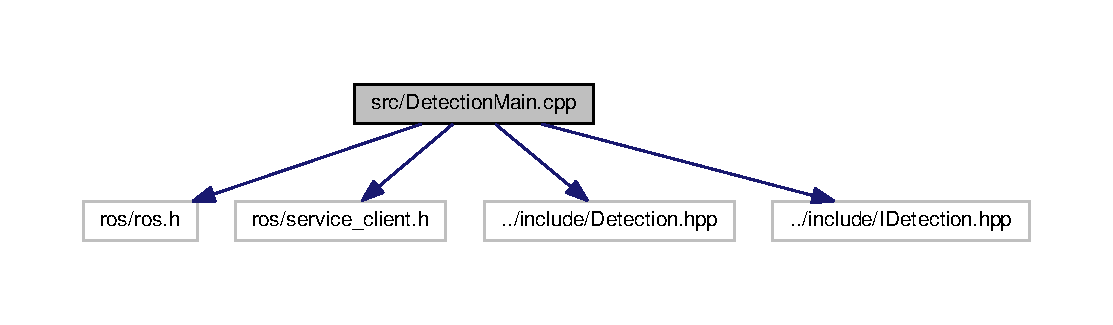
\includegraphics[width=350pt]{_detection_main_8cpp__incl}
\end{center}
\end{figure}
\subsection*{Functions}
\begin{DoxyCompactItemize}
\item 
int \hyperlink{_detection_main_8cpp_a0ddf1224851353fc92bfbff6f499fa97}{main} (int argc, char $\ast$argv\mbox{[}$\,$\mbox{]})
\end{DoxyCompactItemize}


\subsection{Detailed Description}
main file for Detection node 

\begin{DoxyAuthor}{Author}
Kartik Madhira 

Arjun Gupta 

Aruna Baijal 
\end{DoxyAuthor}
\begin{DoxyCopyright}{Copyright}
M\+IT License (c) 2019 Kartik Madhira, Aruna Baijal, Arjun Gupta 
\end{DoxyCopyright}


\subsection{Function Documentation}
\index{Detection\+Main.\+cpp@{Detection\+Main.\+cpp}!main@{main}}
\index{main@{main}!Detection\+Main.\+cpp@{Detection\+Main.\+cpp}}
\subsubsection[{\texorpdfstring{main(int argc, char $\ast$argv[])}{main(int argc, char *argv[])}}]{\setlength{\rightskip}{0pt plus 5cm}int main (
\begin{DoxyParamCaption}
\item[{int}]{argc, }
\item[{char $\ast$}]{argv\mbox{[}$\,$\mbox{]}}
\end{DoxyParamCaption}
)}\hypertarget{_detection_main_8cpp_a0ddf1224851353fc92bfbff6f499fa97}{}\label{_detection_main_8cpp_a0ddf1224851353fc92bfbff6f499fa97}

\hypertarget{main_8cpp}{}\section{src/main.cpp File Reference}
\label{main_8cpp}\index{src/main.\+cpp@{src/main.\+cpp}}
{\ttfamily \#include \char`\"{}../include/\+User\+Interface.\+hpp\char`\"{}}\\*
{\ttfamily \#include \char`\"{}../include/\+Warehouse\+Manager.\+hpp\char`\"{}}\\*
Include dependency graph for main.\+cpp\+:
\nopagebreak
\begin{figure}[H]
\begin{center}
\leavevmode
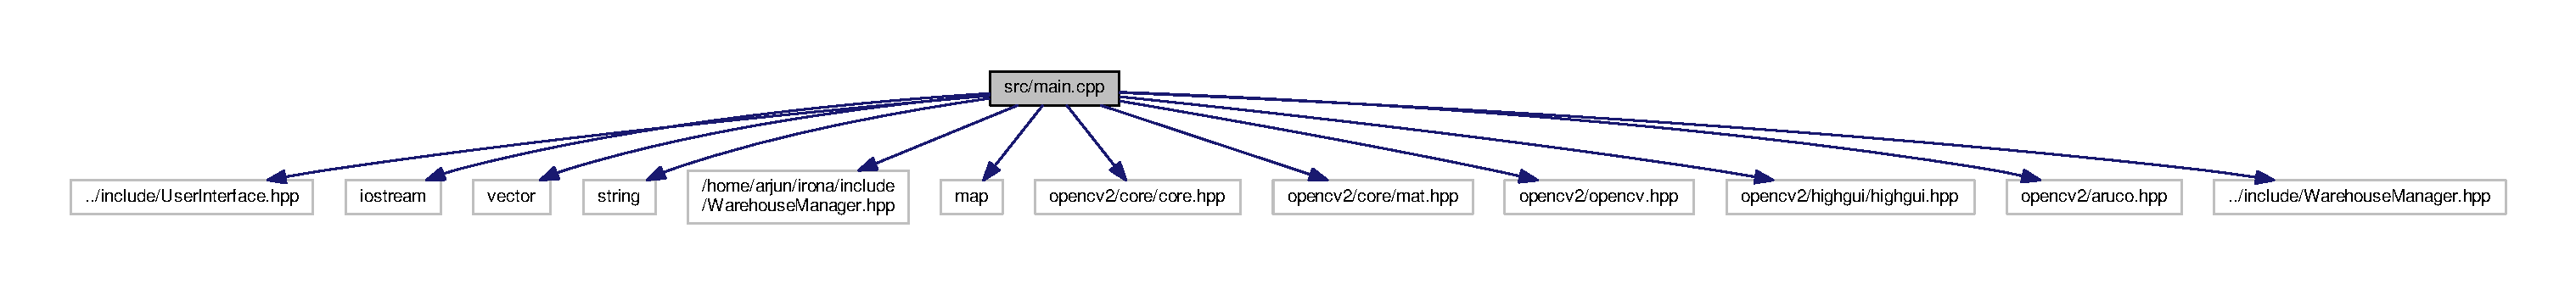
\includegraphics[width=350pt]{main_8cpp__incl}
\end{center}
\end{figure}
\subsection*{Functions}
\begin{DoxyCompactItemize}
\item 
int \hyperlink{main_8cpp_a0ddf1224851353fc92bfbff6f499fa97}{main} (int argc, char $\ast$argv\mbox{[}$\,$\mbox{]})
\end{DoxyCompactItemize}


\subsection{Function Documentation}
\index{main.\+cpp@{main.\+cpp}!main@{main}}
\index{main@{main}!main.\+cpp@{main.\+cpp}}
\subsubsection[{\texorpdfstring{main(int argc, char $\ast$argv[])}{main(int argc, char *argv[])}}]{\setlength{\rightskip}{0pt plus 5cm}int main (
\begin{DoxyParamCaption}
\item[{int}]{argc, }
\item[{char $\ast$}]{argv\mbox{[}$\,$\mbox{]}}
\end{DoxyParamCaption}
)}\hypertarget{main_8cpp_a0ddf1224851353fc92bfbff6f499fa97}{}\label{main_8cpp_a0ddf1224851353fc92bfbff6f499fa97}

\hypertarget{_navigation_8cpp}{}\section{src/\+Navigation.cpp File Reference}
\label{_navigation_8cpp}\index{src/\+Navigation.\+cpp@{src/\+Navigation.\+cpp}}


Navigation class Implementation.  


{\ttfamily \#include \char`\"{}../include/\+Navigation.\+hpp\char`\"{}}\\*
Include dependency graph for Navigation.\+cpp\+:
\nopagebreak
\begin{figure}[H]
\begin{center}
\leavevmode
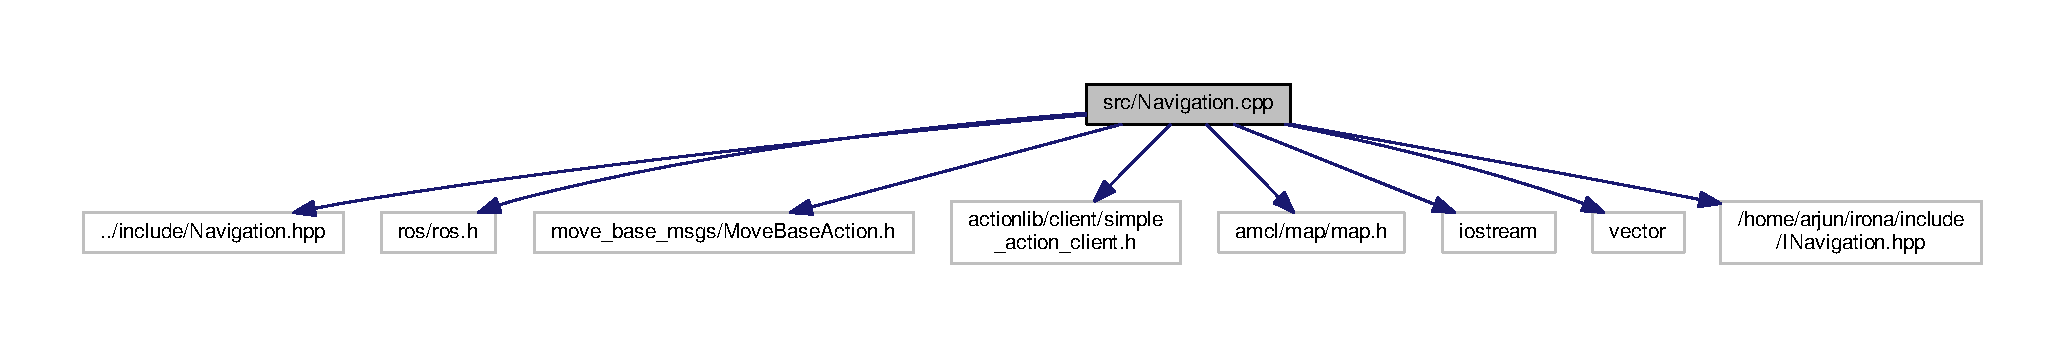
\includegraphics[width=350pt]{_navigation_8cpp__incl}
\end{center}
\end{figure}
\subsection*{Typedefs}
\begin{DoxyCompactItemize}
\item 
typedef actionlib\+::\+Simple\+Action\+Client$<$ move\+\_\+base\+\_\+msgs\+::\+Move\+Base\+Action $>$ \hyperlink{_navigation_8cpp_a21e20cc0b6656ae897b3cbb969b93241}{Move\+Base\+Client}
\end{DoxyCompactItemize}


\subsection{Detailed Description}
Navigation class Implementation. 

\begin{DoxyAuthor}{Author}
Kartik Madhira 

Arjun Gupta 

Aruna Baijal 
\end{DoxyAuthor}
\begin{DoxyCopyright}{Copyright}
M\+IT License (c) 2019 Kartik Madhira, Aruna Baijal, Arjun Gupta 
\end{DoxyCopyright}


\subsection{Typedef Documentation}
\index{Navigation.\+cpp@{Navigation.\+cpp}!Move\+Base\+Client@{Move\+Base\+Client}}
\index{Move\+Base\+Client@{Move\+Base\+Client}!Navigation.\+cpp@{Navigation.\+cpp}}
\subsubsection[{\texorpdfstring{Move\+Base\+Client}{MoveBaseClient}}]{\setlength{\rightskip}{0pt plus 5cm}typedef actionlib\+::\+Simple\+Action\+Client$<$move\+\_\+base\+\_\+msgs\+::\+Move\+Base\+Action$>$ {\bf Move\+Base\+Client}}\hypertarget{_navigation_8cpp_a21e20cc0b6656ae897b3cbb969b93241}{}\label{_navigation_8cpp_a21e20cc0b6656ae897b3cbb969b93241}

\hypertarget{_navigation_main_8cpp}{}\section{src/\+Navigation\+Main.cpp File Reference}
\label{_navigation_main_8cpp}\index{src/\+Navigation\+Main.\+cpp@{src/\+Navigation\+Main.\+cpp}}


main file for Navigation node  


{\ttfamily \#include $<$ros/ros.\+h$>$}\\*
{\ttfamily \#include $<$ros/service\+\_\+client.\+h$>$}\\*
{\ttfamily \#include \char`\"{}../include/\+Navigation.\+hpp\char`\"{}}\\*
Include dependency graph for Navigation\+Main.\+cpp\+:
\nopagebreak
\begin{figure}[H]
\begin{center}
\leavevmode
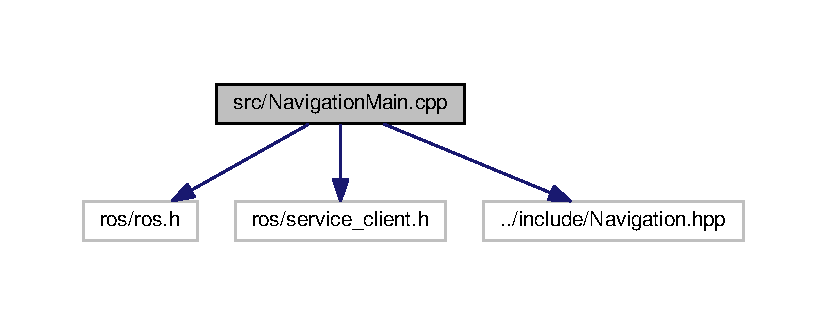
\includegraphics[width=350pt]{_navigation_main_8cpp__incl}
\end{center}
\end{figure}
\subsection*{Functions}
\begin{DoxyCompactItemize}
\item 
int \hyperlink{_navigation_main_8cpp_a0ddf1224851353fc92bfbff6f499fa97}{main} (int argc, char $\ast$argv\mbox{[}$\,$\mbox{]})
\end{DoxyCompactItemize}


\subsection{Detailed Description}
main file for Navigation node 

\begin{DoxyAuthor}{Author}
Kartik Madhira 

Arjun Gupta 

Aruna Baijal 
\end{DoxyAuthor}
\begin{DoxyCopyright}{Copyright}
M\+IT License (c) 2019 Kartik Madhira, Aruna Baijal, Arjun Gupta 
\end{DoxyCopyright}


\subsection{Function Documentation}
\index{Navigation\+Main.\+cpp@{Navigation\+Main.\+cpp}!main@{main}}
\index{main@{main}!Navigation\+Main.\+cpp@{Navigation\+Main.\+cpp}}
\subsubsection[{\texorpdfstring{main(int argc, char $\ast$argv[])}{main(int argc, char *argv[])}}]{\setlength{\rightskip}{0pt plus 5cm}int main (
\begin{DoxyParamCaption}
\item[{int}]{argc, }
\item[{char $\ast$}]{argv\mbox{[}$\,$\mbox{]}}
\end{DoxyParamCaption}
)}\hypertarget{_navigation_main_8cpp_a0ddf1224851353fc92bfbff6f499fa97}{}\label{_navigation_main_8cpp_a0ddf1224851353fc92bfbff6f499fa97}

\hypertarget{_user_interface_8cpp}{}\section{src/\+User\+Interface.cpp File Reference}
\label{_user_interface_8cpp}\index{src/\+User\+Interface.\+cpp@{src/\+User\+Interface.\+cpp}}


Implements User\+Interface class.  


{\ttfamily \#include $<$string.\+h$>$}\\*
{\ttfamily \#include $<$iostream$>$}\\*
{\ttfamily \#include \char`\"{}User\+Interface.\+hpp\char`\"{}}\\*
{\ttfamily \#include \char`\"{}Warehouse\+Manager.\+hpp\char`\"{}}\\*
Include dependency graph for User\+Interface.\+cpp\+:
\nopagebreak
\begin{figure}[H]
\begin{center}
\leavevmode
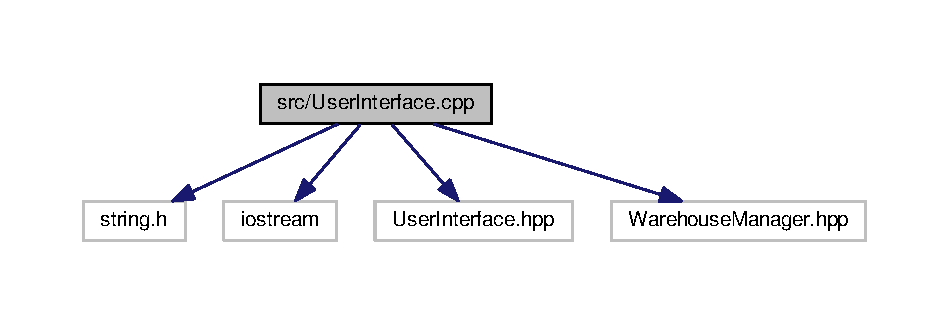
\includegraphics[width=350pt]{_user_interface_8cpp__incl}
\end{center}
\end{figure}


\subsection{Detailed Description}
Implements User\+Interface class. 

\begin{DoxyAuthor}{Author}
Kartik Madhira 

Arjun Gupta 

Aruna Baijal 
\end{DoxyAuthor}
\begin{DoxyCopyright}{Copyright}
M\+IT License (c) 2019 Kartik Madhira, Aruna Baijal, Arjun Gupta 
\end{DoxyCopyright}

\hypertarget{_warehouse_manager_8cpp}{}\section{src/\+Warehouse\+Manager.cpp File Reference}
\label{_warehouse_manager_8cpp}\index{src/\+Warehouse\+Manager.\+cpp@{src/\+Warehouse\+Manager.\+cpp}}


Implements Warehouse\+Manager class.  


{\ttfamily \#include \char`\"{}Warehouse\+Manager.\+hpp\char`\"{}}\\*
{\ttfamily \#include $<$exception$>$}\\*
{\ttfamily \#include $<$string$>$}\\*
Include dependency graph for Warehouse\+Manager.\+cpp\+:
\nopagebreak
\begin{figure}[H]
\begin{center}
\leavevmode
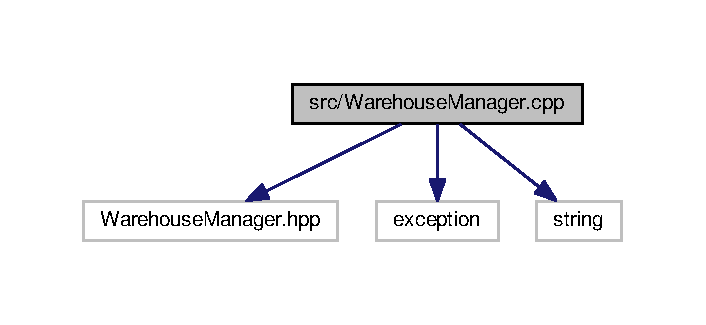
\includegraphics[width=339pt]{_warehouse_manager_8cpp__incl}
\end{center}
\end{figure}


\subsection{Detailed Description}
Implements Warehouse\+Manager class. 

\begin{DoxyAuthor}{Author}
Kartik Madhira 

Arjun Gupta 

Aruna Baijal 
\end{DoxyAuthor}
\begin{DoxyCopyright}{Copyright}
M\+IT License (c) 2019 Kartik Madhira, Aruna Baijal, Arjun Gupta 
\end{DoxyCopyright}

%--- End generated contents ---

% Index
\backmatter
\newpage
\phantomsection
\clearemptydoublepage
\addcontentsline{toc}{chapter}{Index}
\printindex

\end{document}
